%% Figure from MATH 556 notes, section 47 (Lecture 21). ADDED (not from lecture).
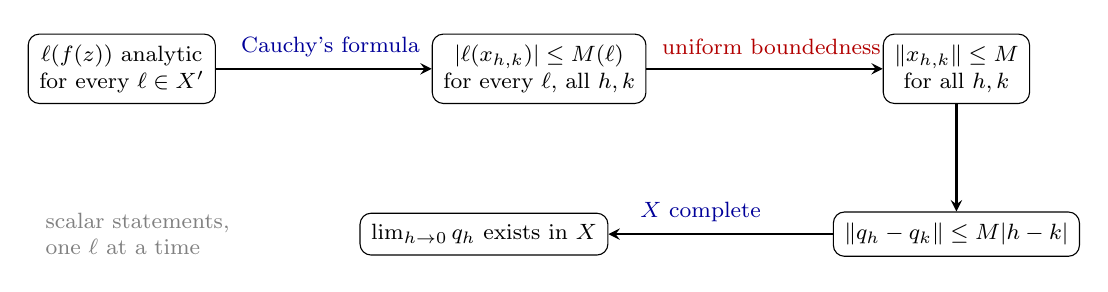
\begin{tikzpicture}[>=stealth, every node/.style={font=\footnotesize}]
    \node[draw, rounded corners, align=center, inner sep=4pt] (a) at (0,0) {$\ell(f(z))$ analytic\\for every $\ell \in X'$};
    \node[draw, rounded corners, align=center, inner sep=4pt] (b) at (5.3,0) {$|\ell(x_{h,k})| \le M(\ell)$\\for every $\ell$, all $h, k$};
    \node[draw, rounded corners, align=center, inner sep=4pt] (c) at (10.6,0) {$\|x_{h,k}\| \le M$\\for all $h, k$};
    \node[draw, rounded corners, align=center, inner sep=4pt] (d) at (10.6,-2.1) {$\|q_h - q_k\| \le M|h - k|$};
    \node[draw, rounded corners, align=center, inner sep=4pt] (e) at (4.6,-2.1) {$\lim_{h \to 0} q_h$ exists in $X$};
    \draw[->, thick] (a) -- (b);
    \draw[->, thick] (b) -- (c);
    \draw[->, thick] (c) -- (d);
    \draw[->, thick] (d) -- (e);
    \node[blue!60!black, align=center] at (2.65,0.28) {Cauchy's formula};
    \node[red!70!black, align=center] at (8.25,0.28) {uniform boundedness};
    \node[blue!60!black] at (7.35,-1.82) {$X$ complete};
    \node[align=left, gray] at (0.2,-2.1) {scalar statements,\\one $\ell$ at a time};
\end{tikzpicture}
